\documentclass[tikz,border=1pt]{standalone}

\usepackage{amsmath}
\usepackage{xcolor}
\usepackage{tikz}
\usepackage{helvet}
\usepackage{pgfplots}

\renewcommand{\familydefault}{\sfdefault}

\usetikzlibrary{arrows.meta}
\usetikzlibrary{calc, fit, matrix, positioning}

\tikzstyle{circ}=[circle, draw, minimum size=0.8cm]
\tikzstyle{square}=[rectangle, draw, minimum size=0.8cm]

\begin{document}

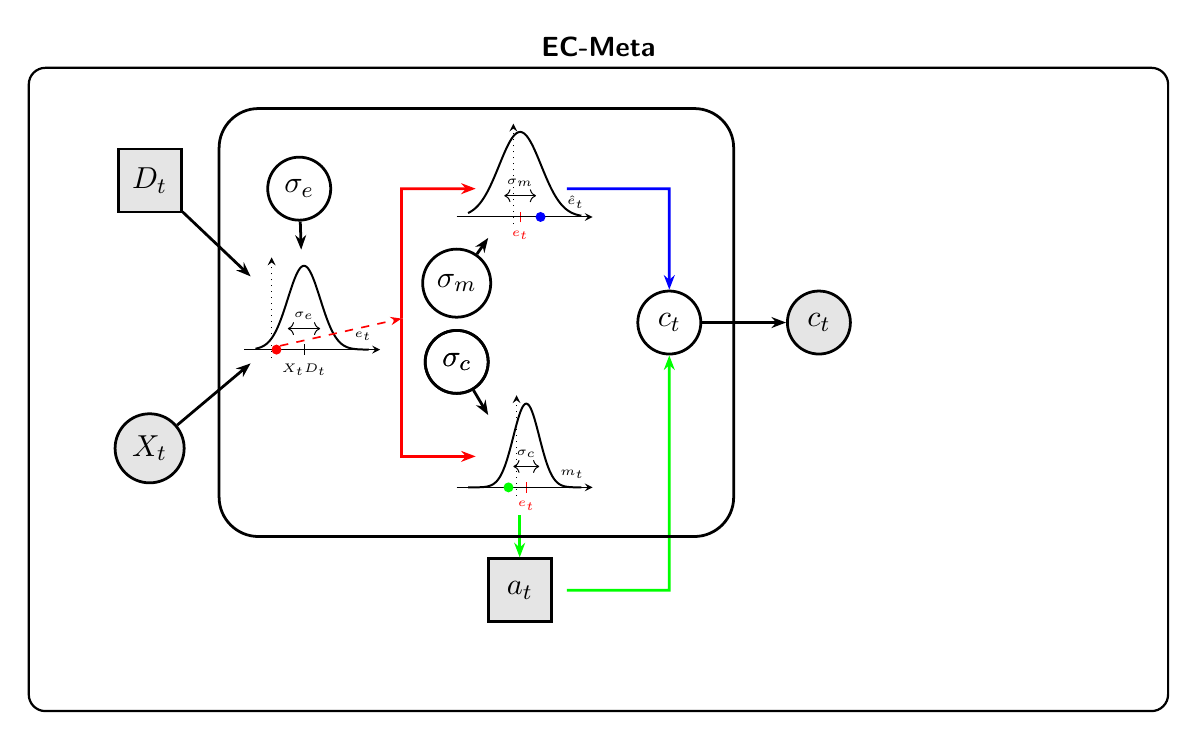
\begin{tikzpicture}


\def\evidencemean{0.3}
\def\evidencesd{1}
\def\ehatmean{1.2}
\def\ehatsd{0.7}
\def\amean{-0.25}
\def\asd{0.4}


% SDT PLOT
\begin{scope}[shift={(-4.5,0.4)}, scale=0.9]
    \pgfplotsset{compat=1.18}

    \begin{axis}[
    width=3.5cm,
    height=3cm,
    xlabel={\tiny $e_t$},
    domain=-1:6,
    samples=100,
    axis lines=middle,
    enlargelimits=true,
    xtick={2},
    xticklabels={\tiny $X_t D_t$},
    x tick style={black},
    xticklabel style={black},
    yticklabels={},
    ytick = \empty,
    y axis line style={dotted},
  ]
    
    % Normal distribution with mean=2, sd=1
    \addplot[thick, smooth] {exp(-(x-2)^2/(2 * \evidencesd ^2)))/sqrt(2*pi * (\evidencesd)^2};
    
    % Label the standard deviation
    \draw[<->] (axis cs:2-\evidencesd,0.1) -- (axis cs:2+\evidencesd,0.1) 
      node[midway, above] {\tiny $\sigma_e$};

    % Sample point - make it a named coordinate
    \fill[red] (axis cs:\evidencemean,0) circle (2pt);
    \coordinate (sample) at (axis cs:\evidencemean,0);
      
  \end{axis}
\end{scope}

% SDT PLOT2
\begin{scope}[shift={(-1.8,2.1)}, scale=0.9]
    \pgfplotsset{compat=1.18}

    \begin{axis}[
    width=3.5cm,
    height=3cm,
    xlabel={\tiny $\hat e_t$},
    domain=-2.0:3.0,
    samples=100,
    axis lines=middle,
    enlargelimits=true,
    xtick={\evidencemean},
    x tick style={red},
    xticklabel style={red},
    xticklabels={\tiny $e_t$},
    ytick = \empty,
    yticklabels={},
    y axis line style={dotted},
  ]
    
    % Normal distribution with mean=0.55, sd=0.5
    \addplot[thick, smooth] {exp(-((x-\evidencemean)^2/(2*(\ehatsd)^2))/sqrt(2*pi*(\ehatsd)^2)};
    
    % Label the standard deviation
    \draw[<->] (axis cs:\evidencemean-\ehatsd,0.25) -- (axis cs:\evidencemean+\ehatsd,0.25) 
      node[midway, above] {\tiny $\sigma_m$};

    % Sample point - make it a named coordinate
    \fill[blue] (axis cs:\ehatmean,0) circle (2pt);
    \coordinate (sample_m) at (axis cs:\ehatmean,0);
      
  \end{axis}
\end{scope}

% SDT PLOT3
\begin{scope}[shift={(-1.8,-1.35)}, scale=0.9]
    \pgfplotsset{compat=1.18}

    \begin{axis}[
    width=3.5cm,
    height=3cm,
    xlabel={\tiny $m_t$},
    domain=-1.5:2,
    samples=100,
    axis lines=middle,
    enlargelimits=true,
    xtick={\evidencemean},
    x tick style={red},
    xticklabel style={red},
    xticklabels={\tiny $e_t$},
    yticklabels={},
    ytick = \empty,
    y axis line style={dotted},
  ]
    
    % Normal distribution with mean=0.55, sd=0.5
    \addplot[thick, smooth] {exp(-((x-\evidencemean)^2/(2*(\asd)^2))/sqrt(2*pi*(\asd)^2)};
    
    % Label the standard deviation
    \draw[<->] (axis cs:\evidencemean-\asd,0.25) -- (axis cs:\evidencemean+\asd,0.25) 
      node[midway, above] {\tiny $\sigma_c$};

    % Sample point - make it a named coordinate
    \fill[green] (axis cs:\amean,0) circle (2pt);
    \coordinate (sample_m) at (axis cs:\amean,0);
      
  \end{axis}
\end{scope}


\tikzset{>={Stealth[scale=0.7]}}
\tikzset{every node/.style={font=\sffamily\fontsize{11pt}{12pt}\selectfont}}
\tikzset{every path/.style={line width=1pt}}

% Main matrix
\matrix (m0) [
    ampersand replacement=\&,
    matrix of math nodes,
    nodes in empty cells,
    column sep=.7cm,
    row sep=0.5cm,
]
{
    |[square, draw, fill=gray!20]| D_t \& 
    |[minimum size=1.2cm, inner sep=0pt, draw=none]| \&
    |[minimum size=1.2cm, inner sep=0pt, draw=none]| \&
    |[minimum size=1.2cm, inner sep=0pt, draw=none]| \&
    |[minimum size=1.2cm, inner sep=0pt, draw=none]| \&
    |[minimum size=1.2cm, inner sep=0pt, draw=none]| \&
    |[minimum size=1.2cm, inner sep=0pt, draw=none]| \\
    |[minimum size=1.2cm, inner sep=0pt, draw=none]| \&
    |[minimum size=1.2cm, inner sep=0pt, draw=none]| \&
    |[minimum size=1.2cm, inner sep=0pt, draw=none]| \&
    |[minimum size=1.2cm, inner sep=0pt, draw=none]| \&
    |[minimum size=1.2cm, inner sep=0pt, draw=none]| \&
    |[minimum size=1.2cm, inner sep=0pt, draw=none]| \\
    |[circ, draw, fill=gray!20]| X_t \&
    |[minimum size=1.2cm, inner sep=0pt, draw=none]| \&
    |[minimum size=1.2cm, inner sep=0pt, draw=none]| \&
    |[minimum size=1.2cm, inner sep=0pt, draw=none]| \&
    |[minimum size=1.2cm, inner sep=0pt, draw=none]| \\
    |[minimum size=1.2cm, inner sep=0pt, draw=none]| \&
    |[minimum size=1.2cm, inner sep=0pt, draw=none]| \&
    |[minimum size=1.2cm, inner sep=0pt, draw=none]| \&
    |[minimum size=1.2cm, inner sep=0pt, draw=none]| \&
    |[minimum size=1.2cm, inner sep=0pt, draw=none]|  \\
};

% Two circles between f_t and m_t
\node[circ, draw] (sigma_m) at ($(m0-1-4)!0.5!(m0-4-4) + (-1.8,0.85+0.5)$) {$\sigma_m$};
\node[circ, draw] (sigma_c) at ($(m0-1-4)!0.5!(m0-4-4) + (-1.8,+0.85-0.5)$) {$\sigma_c$};

\node[circ, draw] (sigma_e) at ($(m0-1-2)$) {$\sigma_e$};

\node[circ, draw] (sigma_c) at ($(m0-1-4)!0.5!(m0-4-4) + (-1.8,+0.85-0.5)$) {$\sigma_c$};

\node[square, draw, fill=gray!20] (a_t) at ($(m0-4-4)!0.5!(m0-4-4) + (-1,0)$) {$a_t$};

% New c_t nodes shifted 1cm to the left
\node[circ, draw] (ct1) at ($(m0-2-5) + (-1,0)$) {$c_t$};
\node[circ, draw, fill=gray!20] (ct2) at ($(m0-2-6) + (-1,0)$) {$c_t$};


% Arrows
\draw[->] (m0-1-1) -- (m0-2-2);
\draw[->] (m0-3-1) -- (m0-2-2);
%\draw[->] (m0-3-4) -- (m0-4-4);
\draw[->] (ct1) -- (ct2);

\coordinate (sigma_m_end) at (-1, 2.5);
\coordinate (sigma_c_end) at (-1, -1);
\coordinate (sigma_e_end) at (-3.75, 1);


\draw[->] (sigma_m) -- ($(sigma_m)!0.5!(sigma_m_end)$);
\draw[->] (sigma_c) -- ($(sigma_c)!0.5!(sigma_c_end)$);
\draw[->] (sigma_e) -- ($(sigma_e)!0.5!(sigma_e_end)$);

\coordinate (start_point) at (-1, -1.6);
\draw[->, green] (start_point) -- (a_t.north);



% Split point closer to distribution
\coordinate (split) at (-2.5, 0.9);

% Arrow from sample to split point
\draw[->, red, dashed, line width=0.6pt] (sample) -- (split);


% From split to f_t and m_t with right angles - stopping halfway
\coordinate (turn_up) at (-2.5, 2.55);
\coordinate (turn_down) at (-2.5, -0.85);
\draw[->, red] (split) -- (turn_up) -- ($(turn_up)!0.5!(m0-1-4.west)$);
\draw[->, red] (split) -- (turn_down) -- ($(turn_down)!0.5!(m0-3-4.west)$);


% Split point closer to distribution
\coordinate (split2) at (-0.4, 2.55);
\coordinate (turn_down2) at (0.9, 2.55);
\draw[->, blue] (split2) -- (turn_down2) -- ($(turn_down2)!1!(ct1.north)$);

\coordinate (split3) at (-0.4, -2.55);
\coordinate (turn_up2) at (0.9, -2.55);
\draw[->, green] (split3) -- (turn_up2) -- ($(turn_up2)!1!(ct1.south)$);


% Trial plate
\pgfsetcornersarced{\pgfpoint{5mm}{5mm}}
\node[draw=black, fit=(m0-1-2) (m0-3-4) (ct1), inner sep=4mm] {};

\node[
  draw,
  thick,
  rounded corners=6pt,
  fit=(m0),
  inner sep=8mm,
  label={[font=\bfseries]above: EC-Meta},
  name=wholemodel
] {};

\end{tikzpicture}
\end{document}